\chapter{De Jiuzhaigou à Chengdu}
\section*{29 septembre 2015}
Jiuzhaigou est une réserve naturelle qui comprend 2 vallées avec des cascades et des lacs aux couleurs étonnantes \newline
 \newline
\centerline{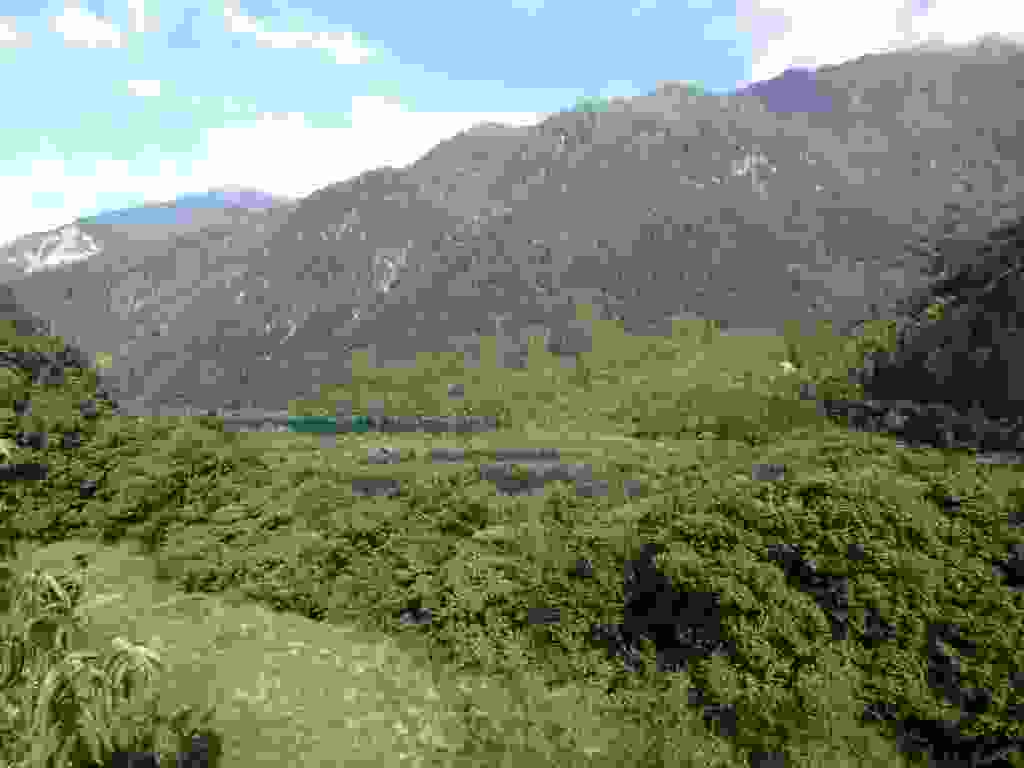
\includegraphics[width=\mywidth]{../wp-content/uploads/2015/09/P9156943-1024x768.jpg} } 
 \newline
 \newline
\centerline{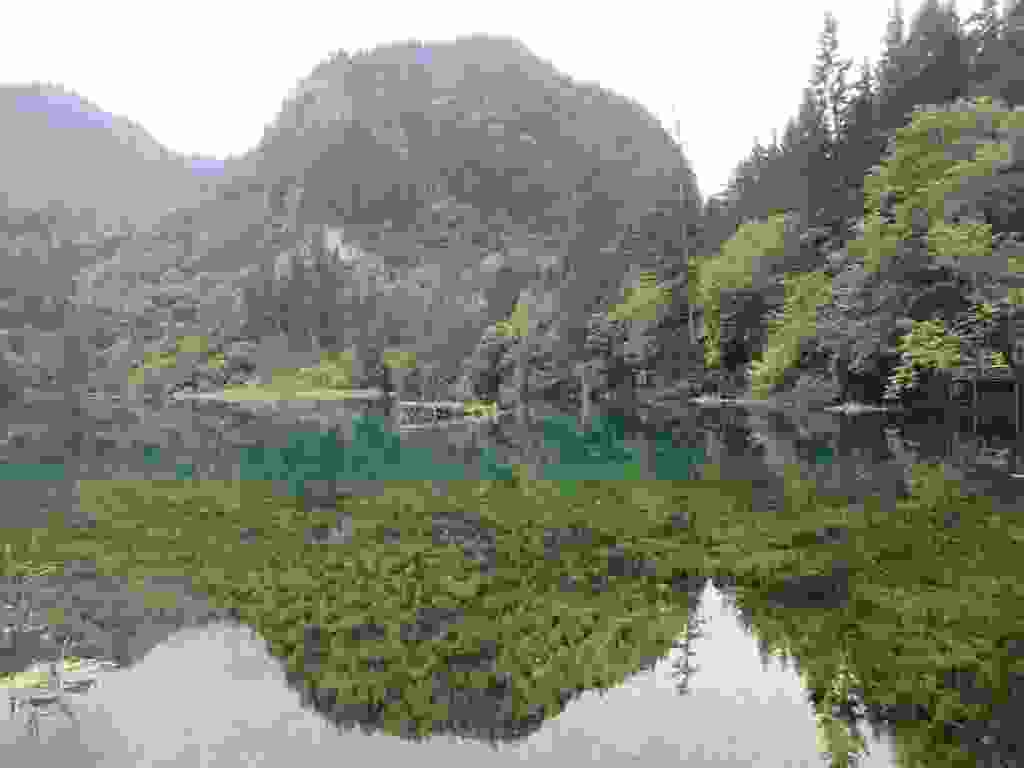
\includegraphics[width=\mywidth]{../wp-content/uploads/2015/09/P9156903-1024x768.jpg} } 
 \newline
 \newline
\centerline{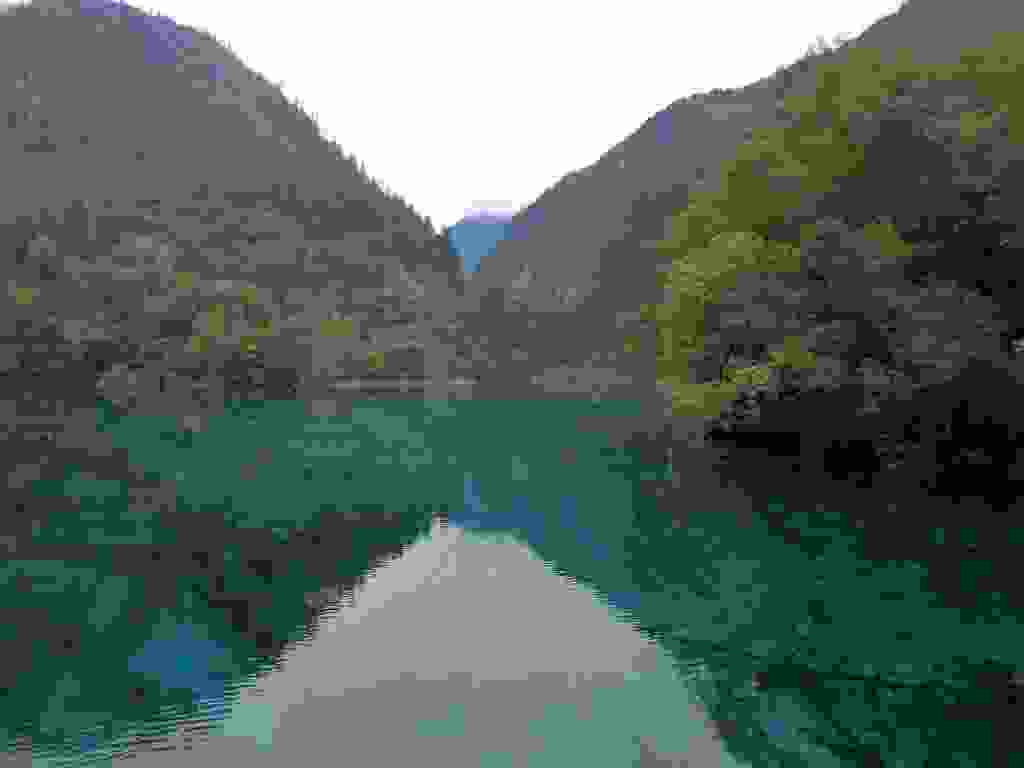
\includegraphics[width=\mywidth]{../wp-content/uploads/2015/09/P9156906-1024x768.jpg} } 
 \newline
 \newline
\centerline{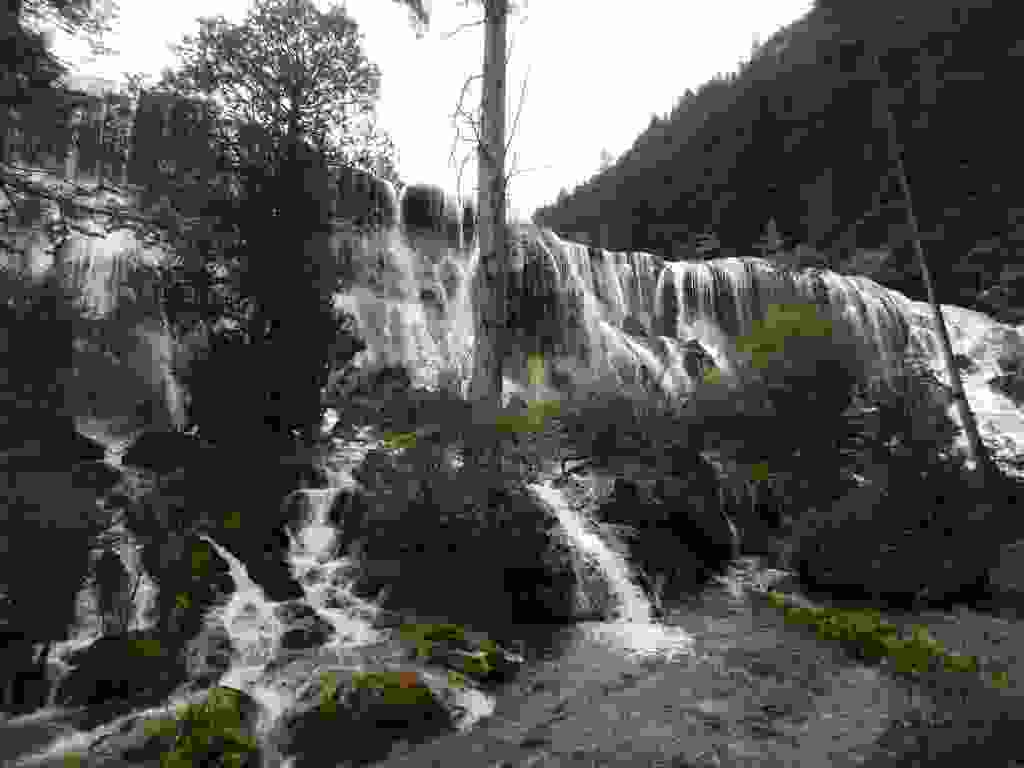
\includegraphics[width=\mywidth]{../wp-content/uploads/2015/09/P9156911-1024x768.jpg} } 
 \newline
 \newline
\centerline{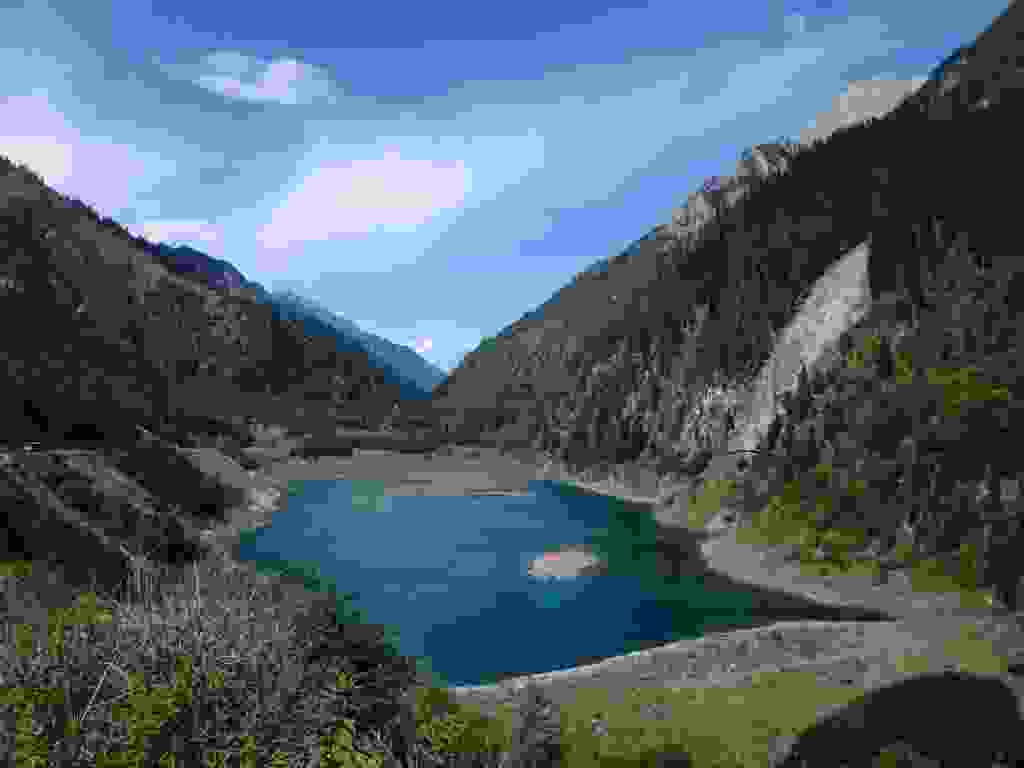
\includegraphics[width=\mywidth]{../wp-content/uploads/2015/09/P9156933-1024x768.jpg} } 
 \newline
 \newline
\centerline{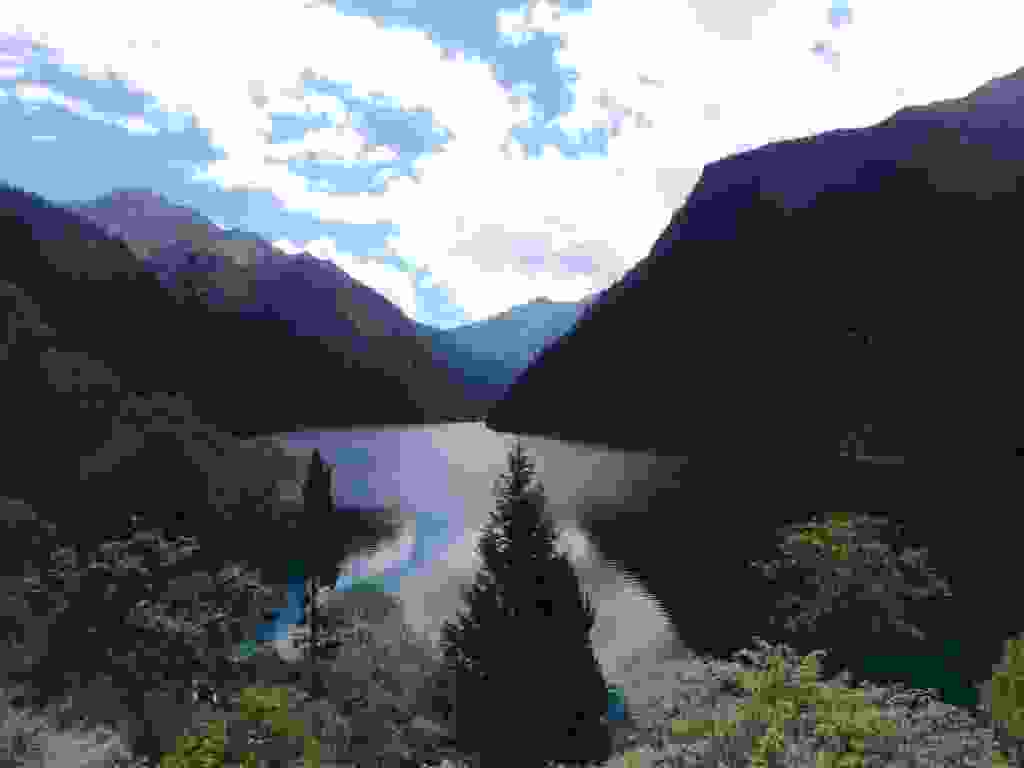
\includegraphics[width=\mywidth]{../wp-content/uploads/2015/09/P9156918-1024x768.jpg} } 
 \newline
 \newline
\centerline{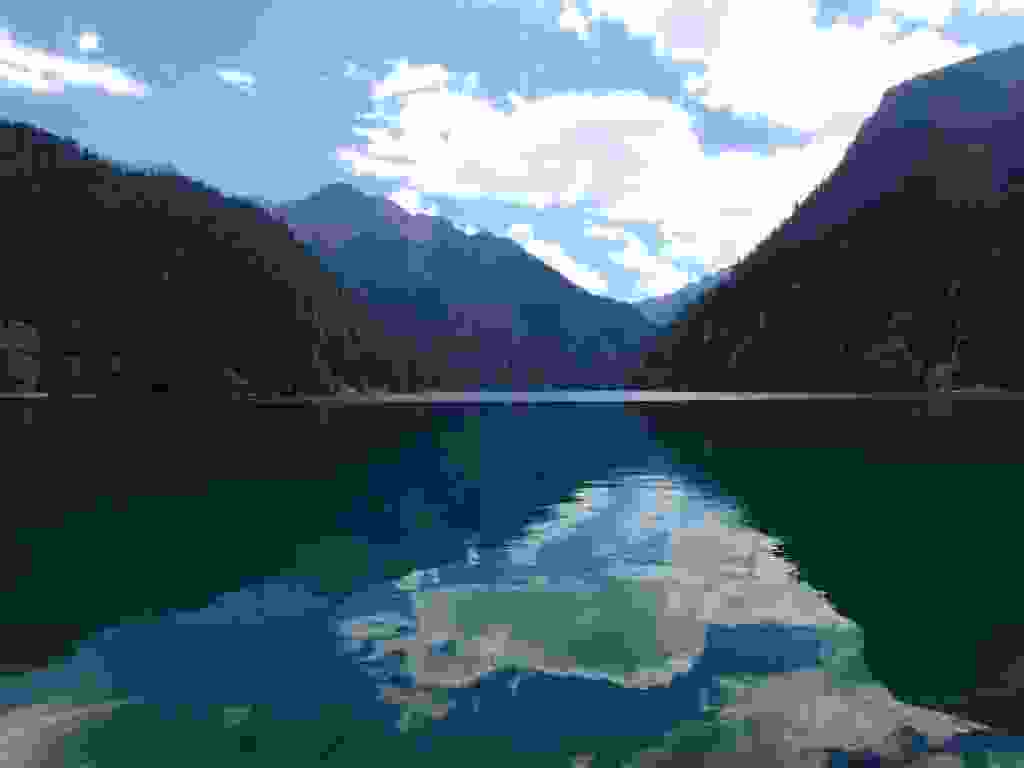
\includegraphics[width=\mywidth]{../wp-content/uploads/2015/09/P9156924-1024x768.jpg} } 
 \newline
 \newline
\centerline{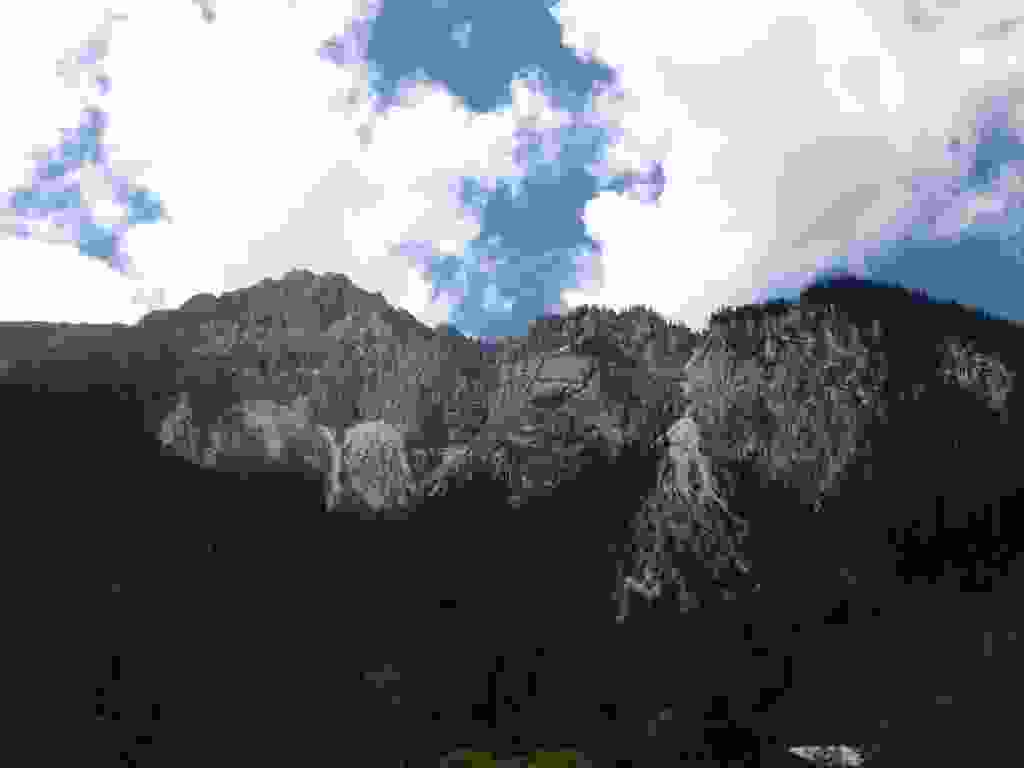
\includegraphics[width=\mywidth]{../wp-content/uploads/2015/09/P9156920-1024x768.jpg} } 
 \newline
 Le site est assez reculé dans les montagnes, pourtant des milliers de personnes le visitent chaque jour \newline
 \newline
\centerline{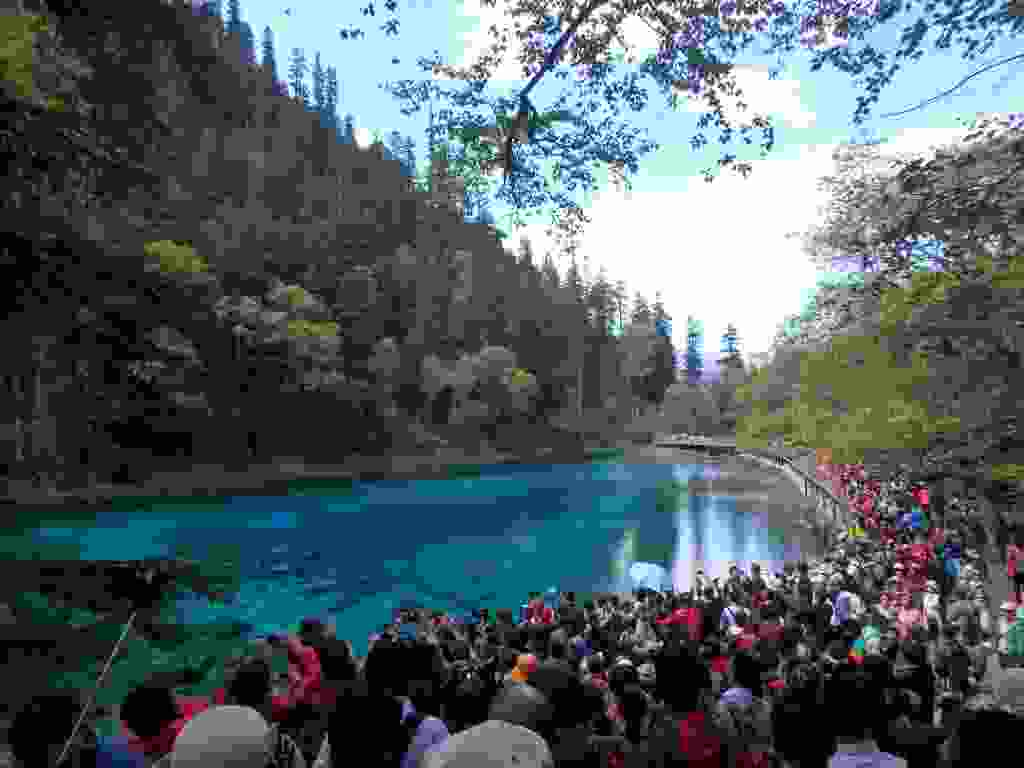
\includegraphics[width=\mywidth]{../wp-content/uploads/2015/09/P9156928-1024x768.jpg} } 
 \newline
 En partant de Jiuzhaigou, plus de 50km de montée pour entrer dans la région tibétaine d'Aba, province du Sichuan. \newline
 \newline
\centerline{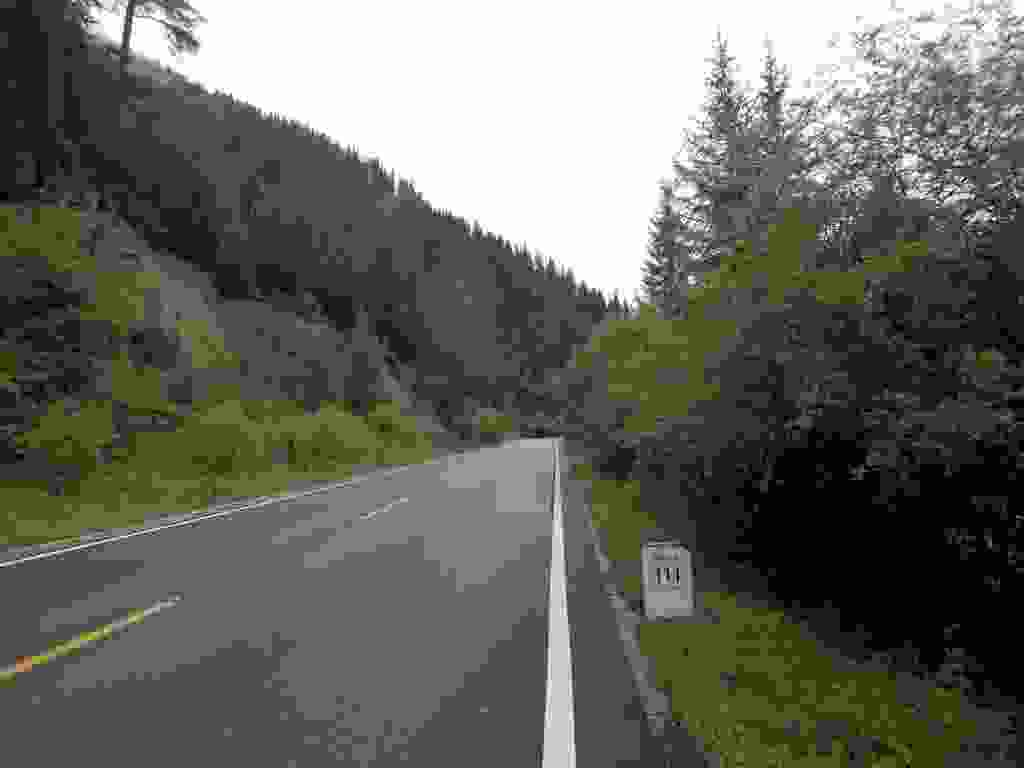
\includegraphics[width=\mywidth]{../wp-content/uploads/2015/09/wpid-p9166957-1024x768.jpg} } 
 \newline
 \newline
\centerline{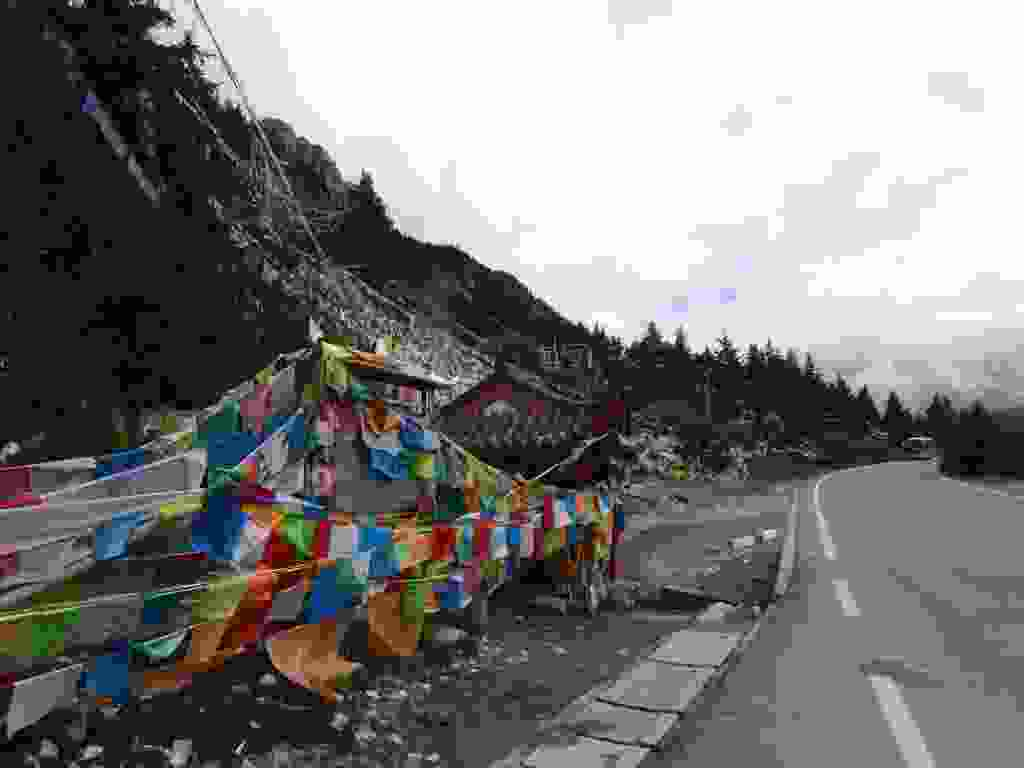
\includegraphics[width=\mywidth]{../wp-content/uploads/2015/09/wpid-p9176966-1024x768.jpg} } 
 \newline
 Restaurant bien décoré \newline
 \newline
\centerline{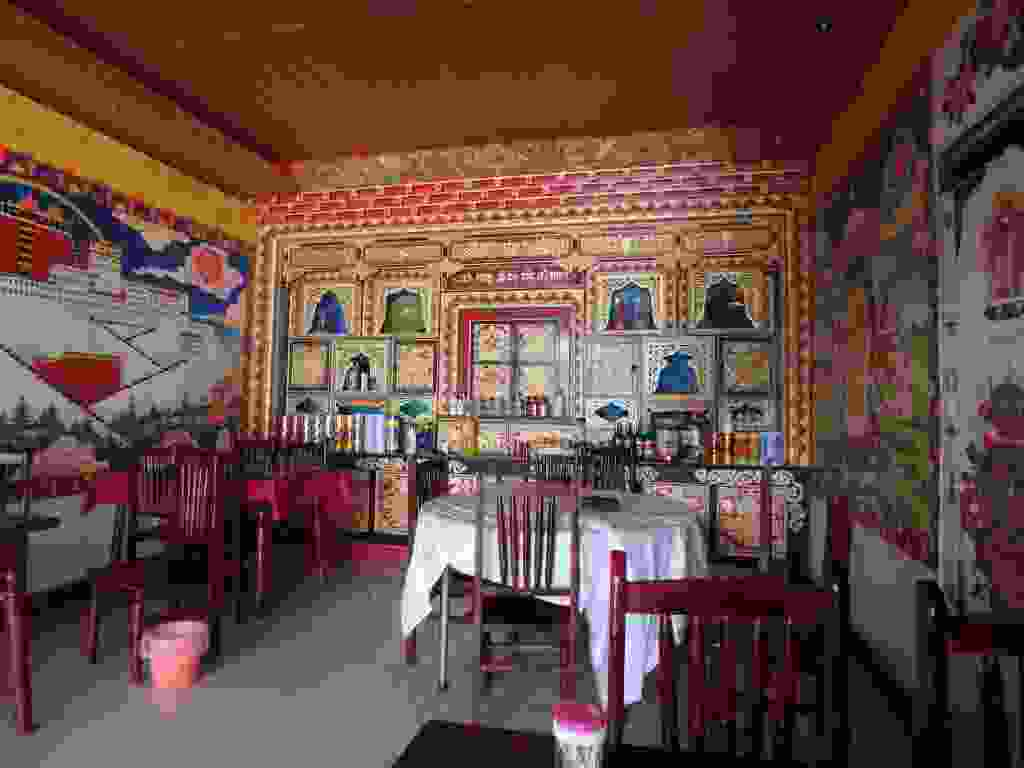
\includegraphics[width=\mywidth]{../wp-content/uploads/2015/09/P9146872-1024x768.jpg} } 
 \newline
 Temple bouddhiste et moulins à prières \newline
 \newline
\centerline{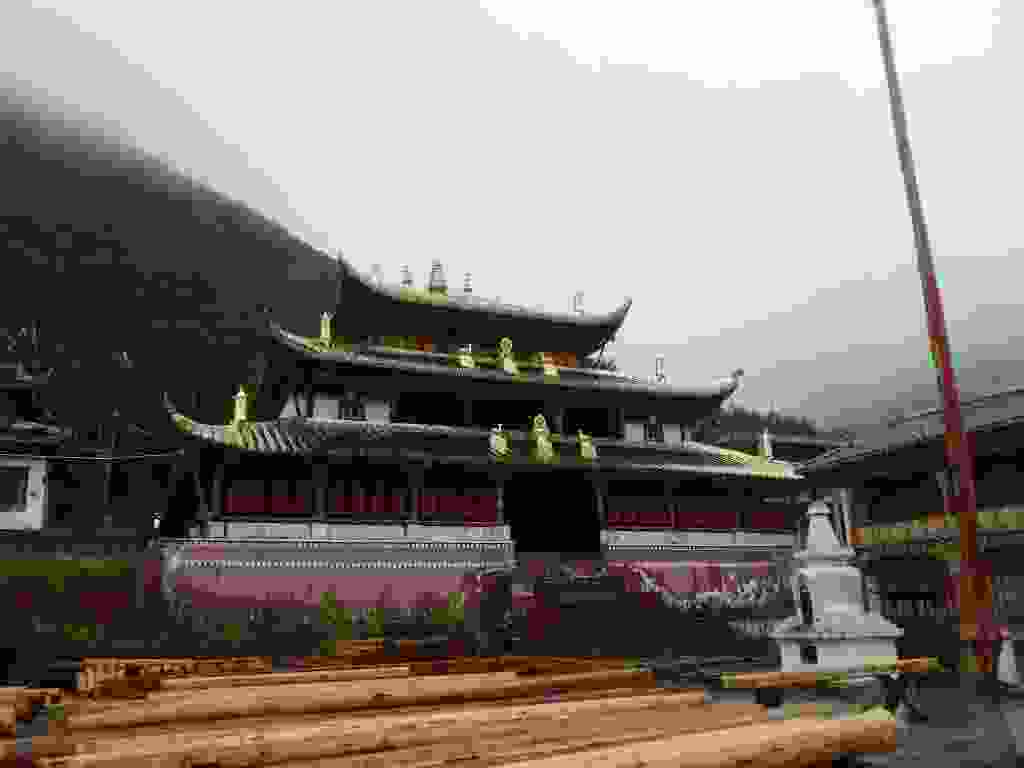
\includegraphics[width=\mywidth]{../wp-content/uploads/2015/09/wpid-p9166946-1024x768.jpg} } 
 \newline
 \newline
\centerline{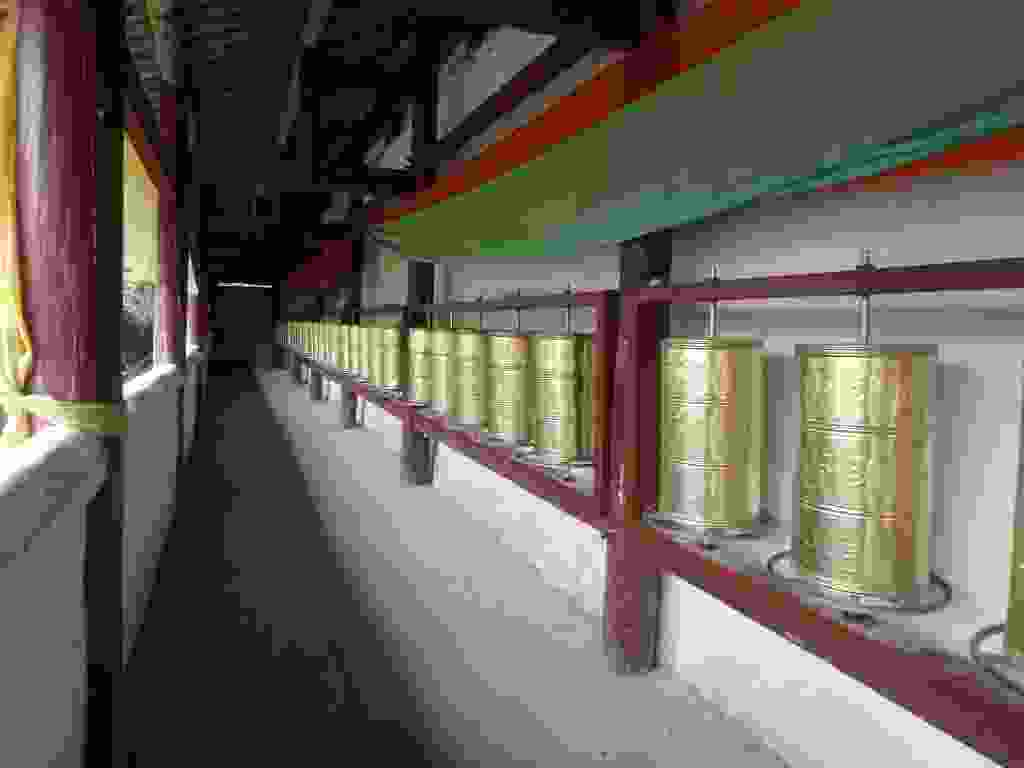
\includegraphics[width=\mywidth]{../wp-content/uploads/2015/09/wpid-p9166948-1024x768.jpg} } 
 \newline
 Troupeaux de yaks sur le plateau \newline
 \newline
\centerline{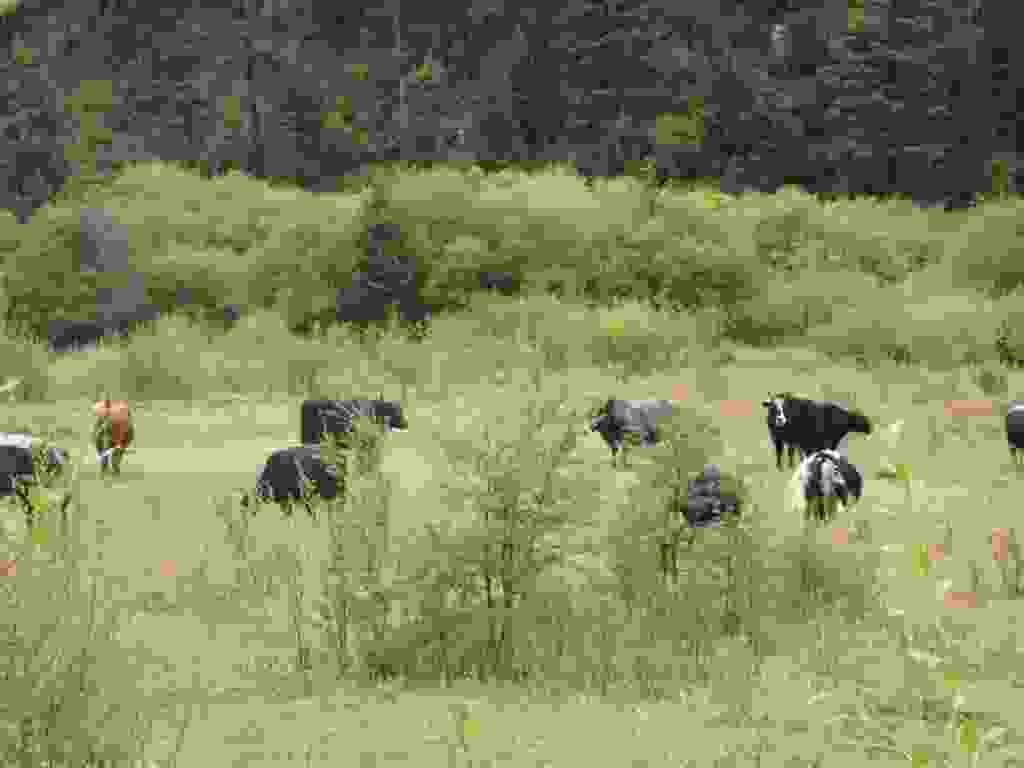
\includegraphics[width=\mywidth]{../wp-content/uploads/2015/09/wpid-p9166956-1024x768.jpg} } 
 \newline
 Après une journée complète sous la pluie je m'arrête pour boire un thé dans un petit stand. Je me retrouve invité à me réchauffer près du poêle, avec brochettes de yak, soupe et thé tibétain \newline
 \newline
\centerline{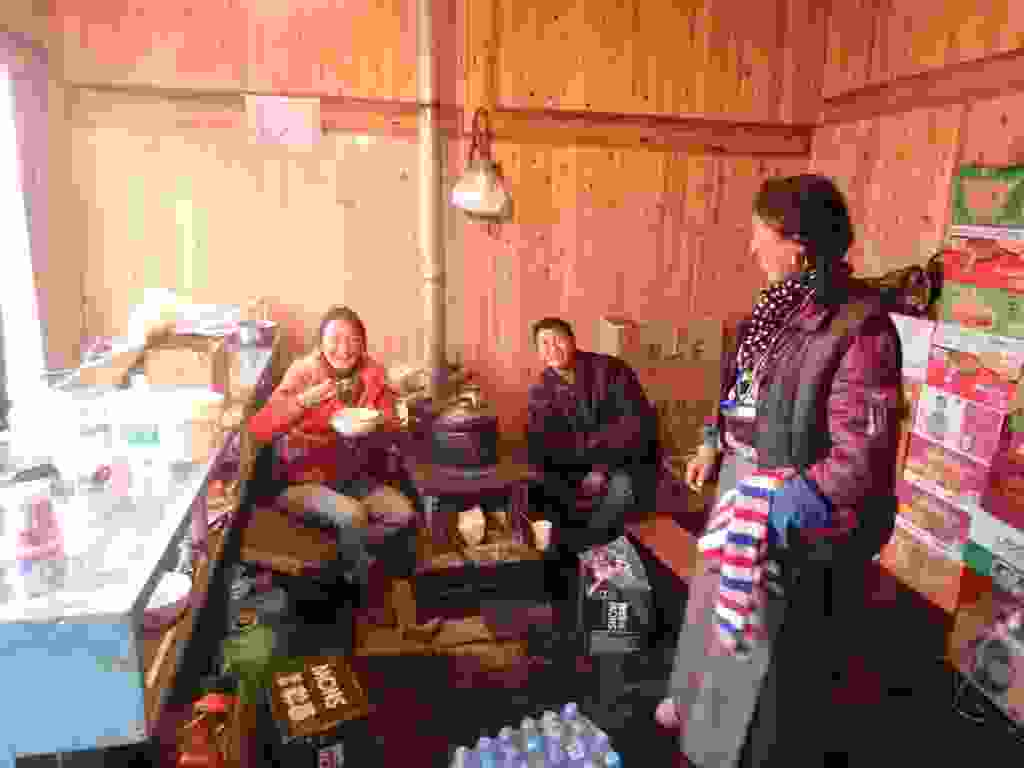
\includegraphics[width=\mywidth]{../wp-content/uploads/2015/09/wpid-p9166963-1024x768.jpg} } 
 \newline
 Les 3 journées suivantes sont en descente le long d'une rivière, en traversant des petits villages \newline
 \newline
\centerline{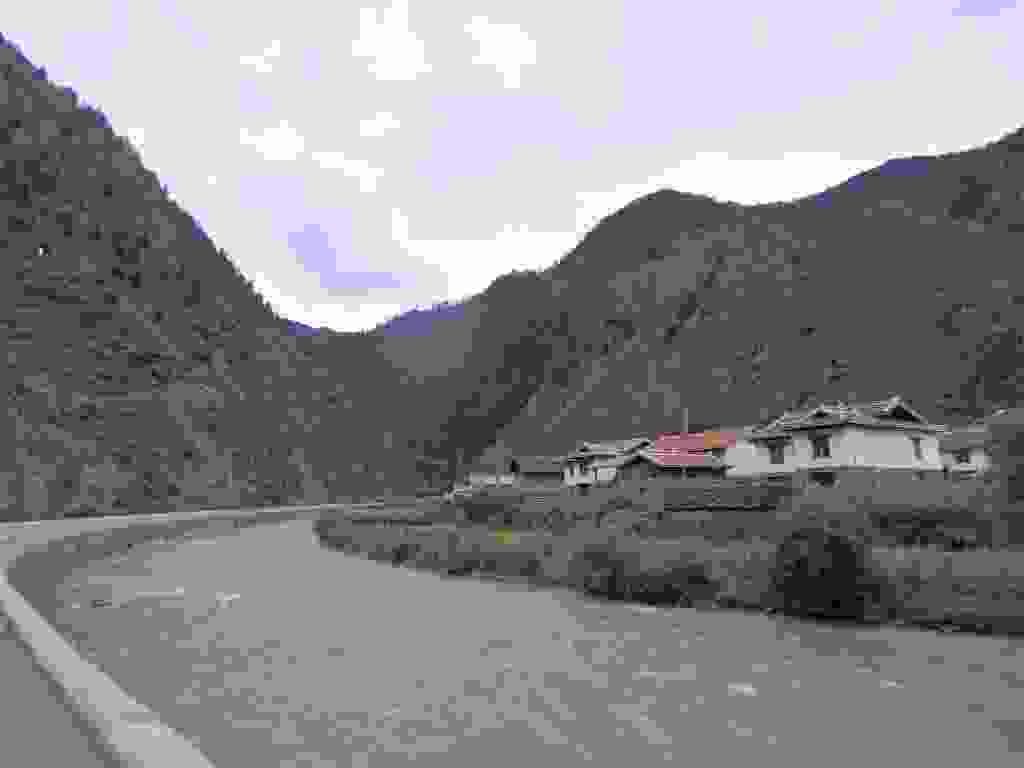
\includegraphics[width=\mywidth]{../wp-content/uploads/2015/09/wpid-p9176984-1024x768.jpg} } 
 \newline
 \newline
\centerline{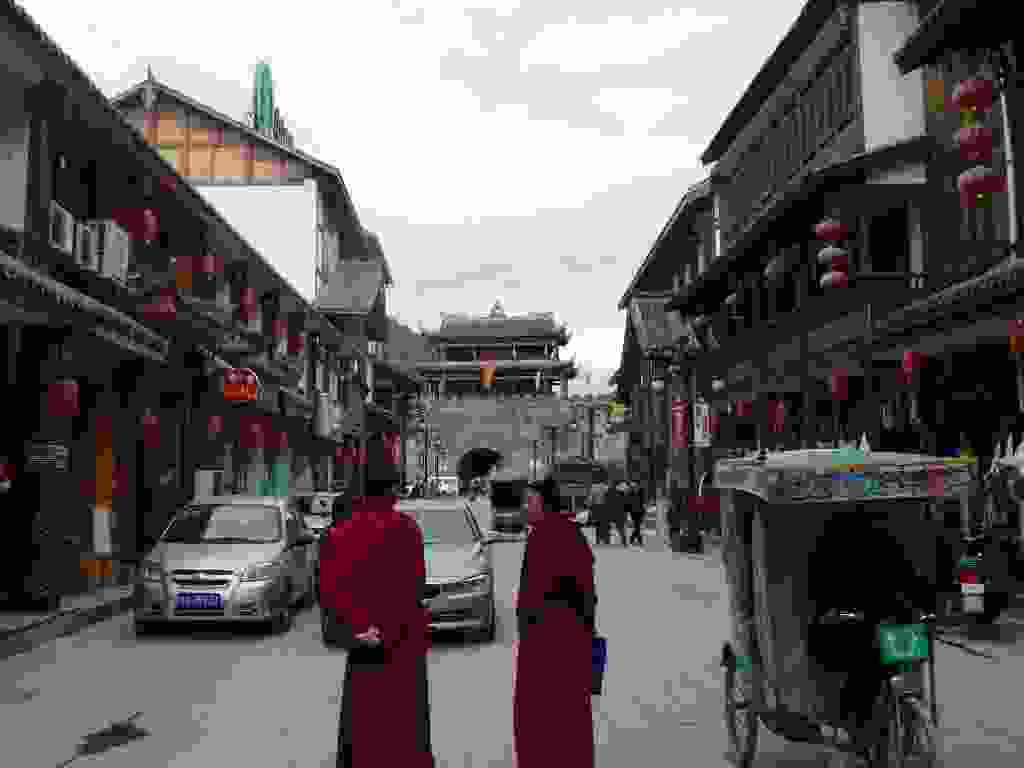
\includegraphics[width=\mywidth]{../wp-content/uploads/2015/09/wpid-p9176978-1024x768.jpg} } 
 \newline
 \newline
\centerline{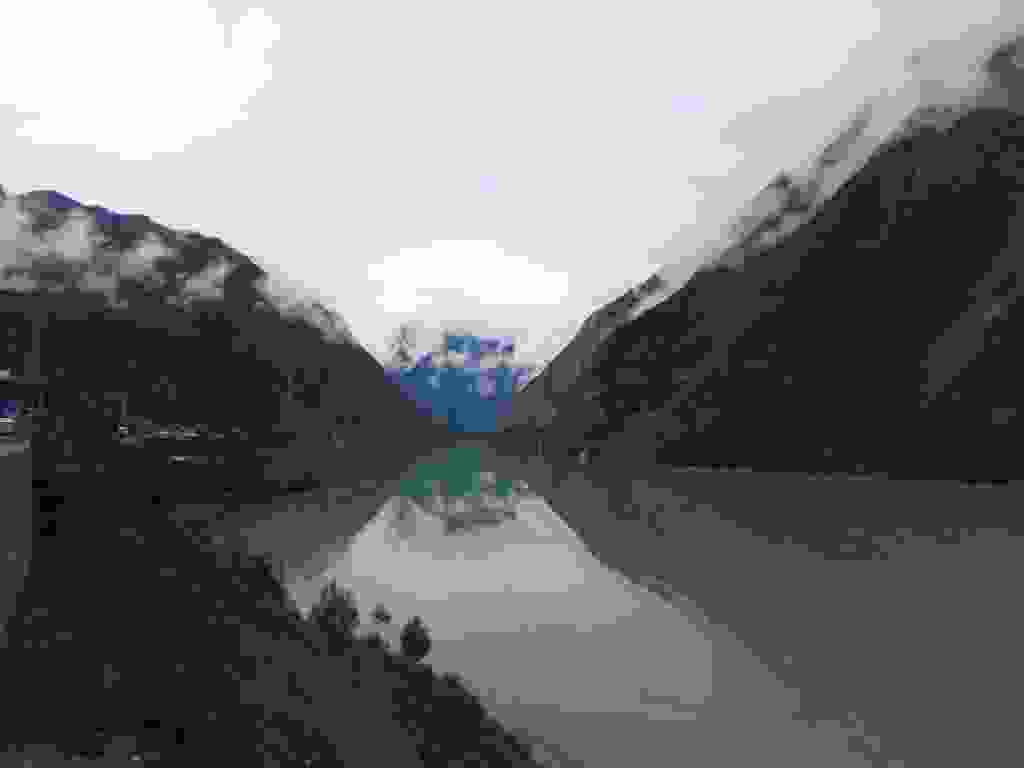
\includegraphics[width=\mywidth]{../wp-content/uploads/2015/09/wpid-p9186991-1024x768.jpg} } 
 \newline
 Un autre temple dans lequel je peux rentrer \newline
 \newline
\centerline{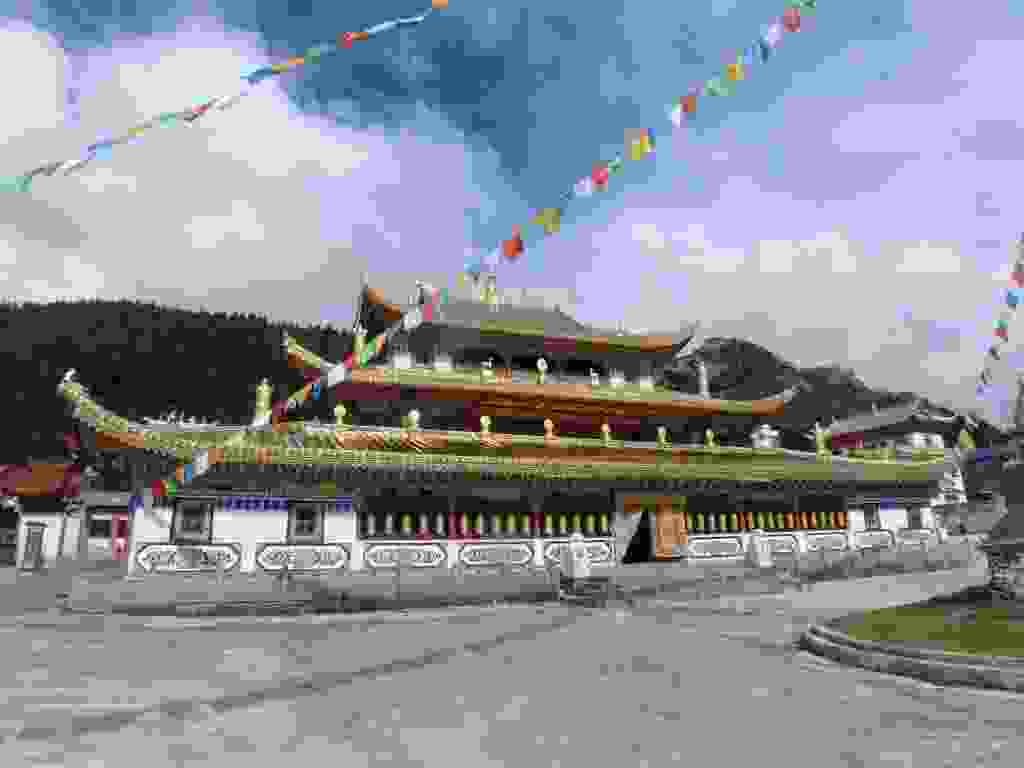
\includegraphics[width=\mywidth]{../wp-content/uploads/2015/09/wpid-p9176968-1024x768.jpg} } 
 \newline
 \newline
\centerline{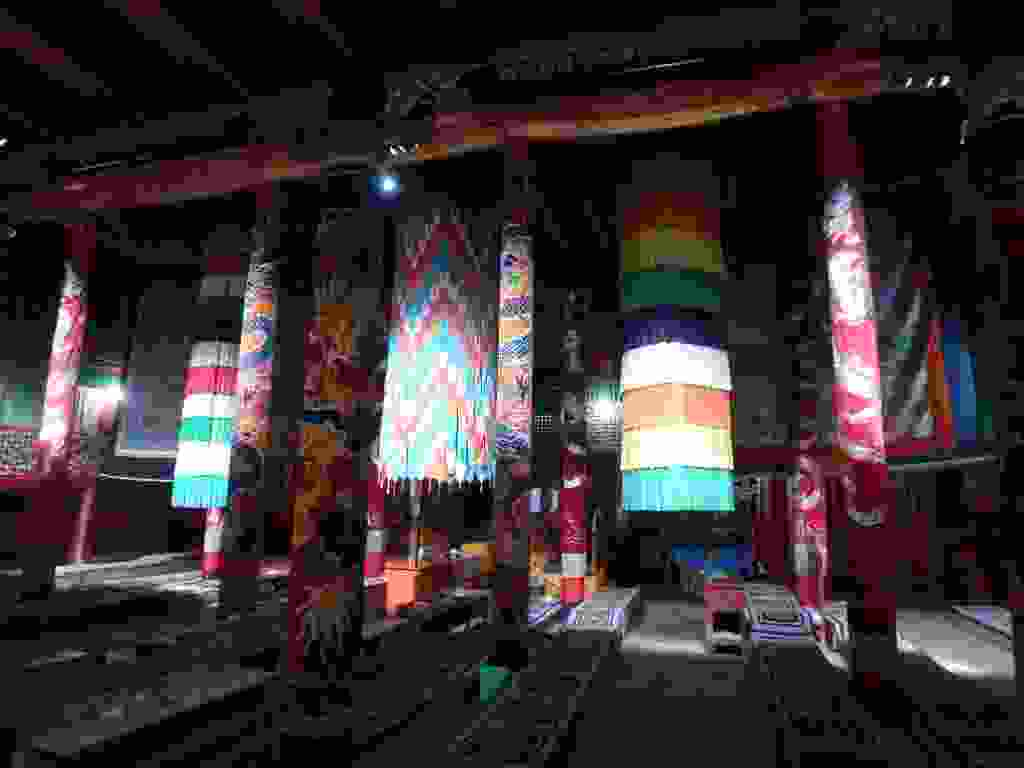
\includegraphics[width=\mywidth]{../wp-content/uploads/2015/09/wpid-p9176970-1024x768.jpg} } 
 \newline
 Trafic important avec chaque jour des centaines de bus de tourisme \newline
 \newline
\centerline{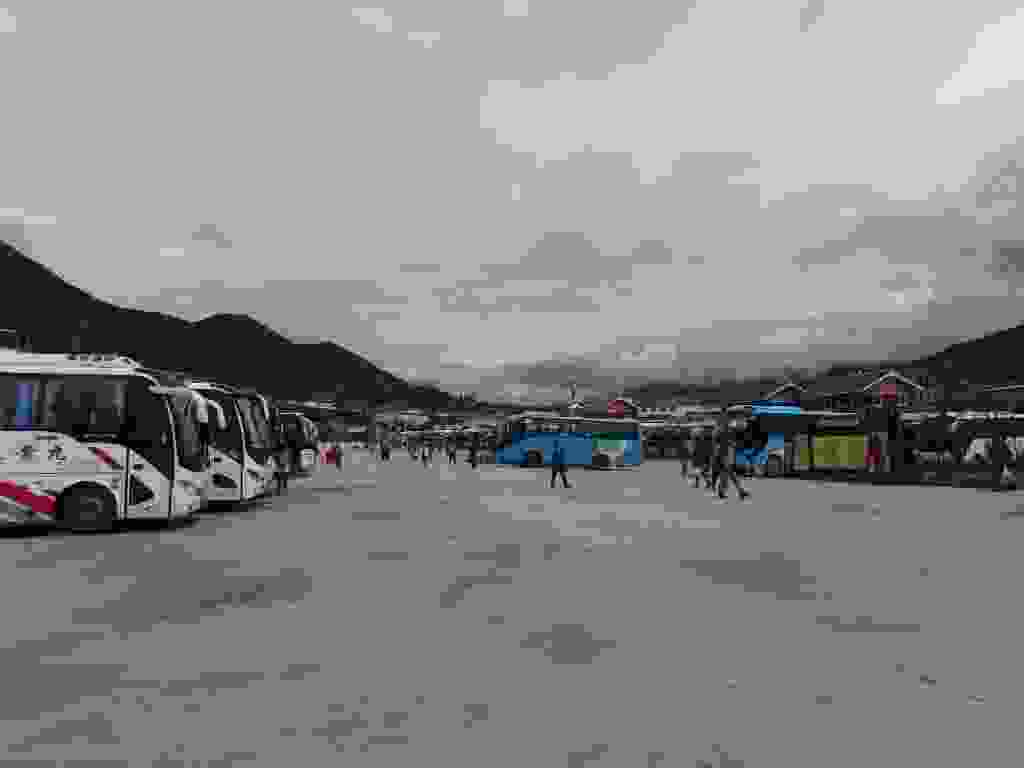
\includegraphics[width=\mywidth]{../wp-content/uploads/2015/09/wpid-p9176972-1024x768.jpg} } 
 \newline
 Passage obligé sur l'autoroute, une partie de la nationale n'a pas été reconstruite après le tremblement de terre de 2008 \newline
 \newline
\centerline{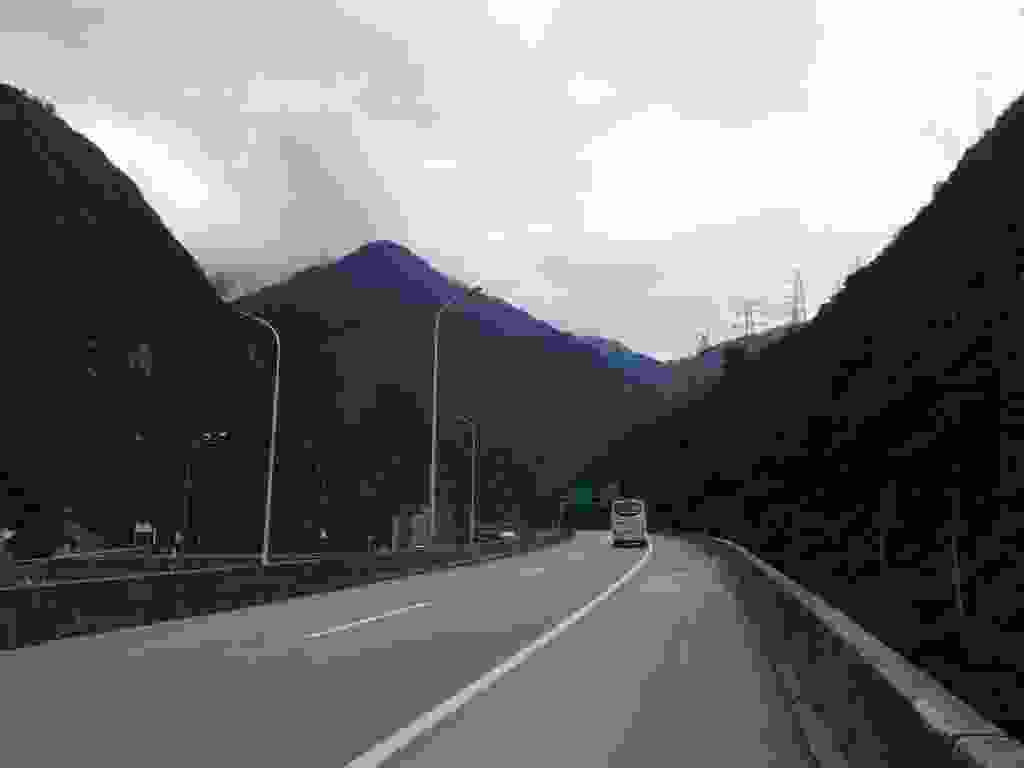
\includegraphics[width=\mywidth]{../wp-content/uploads/2015/09/wpid-p9197010-1024x768.jpg} } 
 \newline
 \newline
\centerline{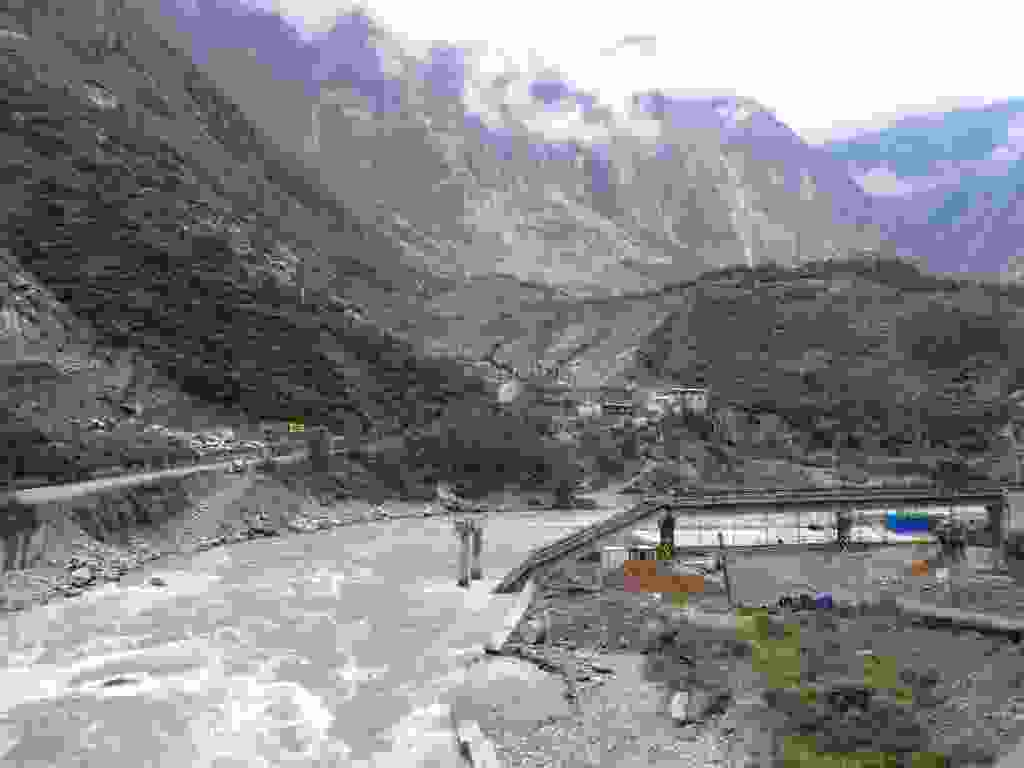
\includegraphics[width=\mywidth]{../wp-content/uploads/2015/09/wpid-p91970091-1024x768.jpg} } 
 \newline
 \newline
\centerline{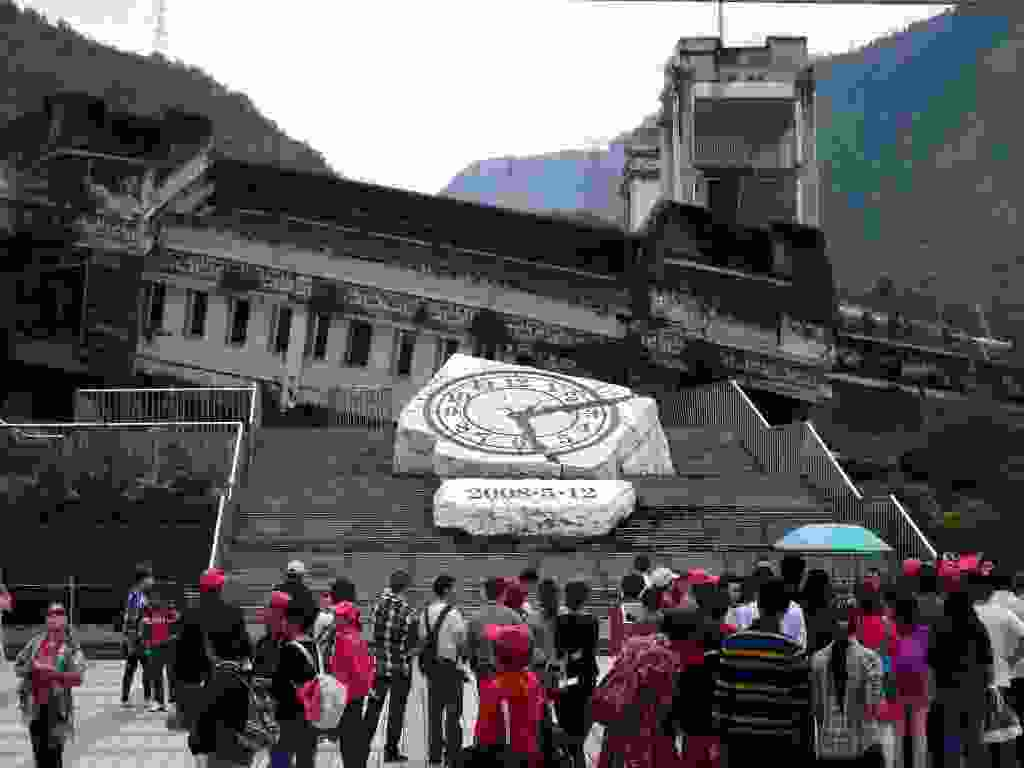
\includegraphics[width=\mywidth]{../wp-content/uploads/2015/09/wpid-p91970121-1024x768.jpg} } 
 \newline
 Contournement d'un grand lac avant d'arriver à Dujiangyian \newline
 \newline
\centerline{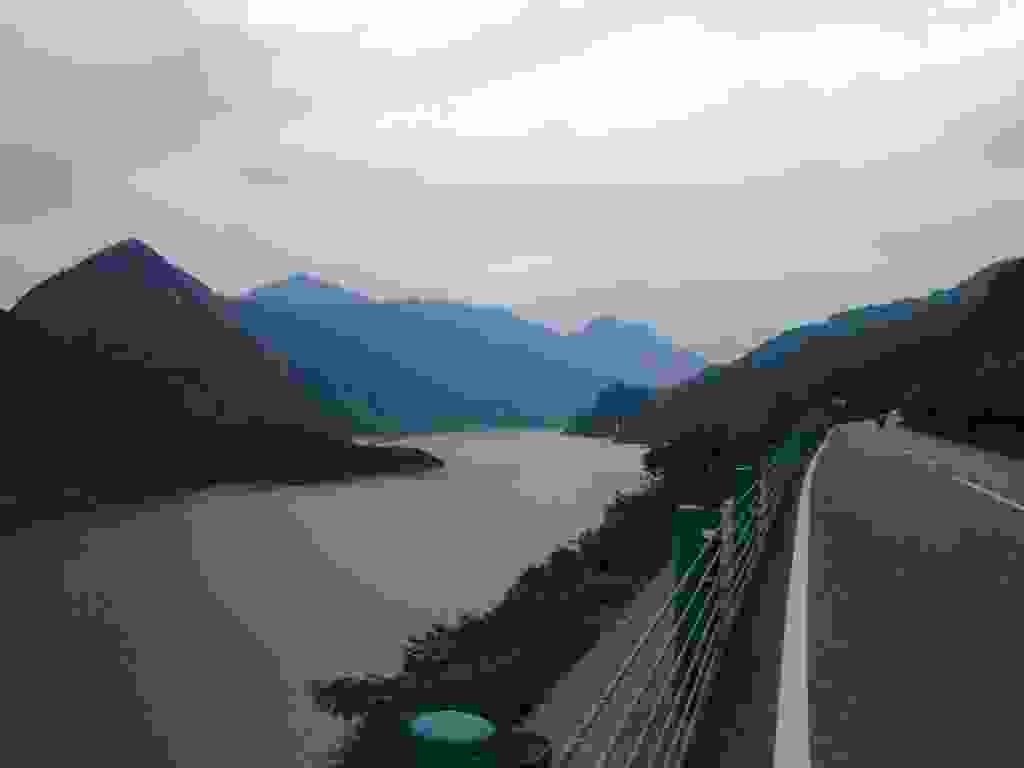
\includegraphics[width=\mywidth]{../wp-content/uploads/2015/09/wpid-p9197016-1024x768.jpg} } 
 \newline
 \newline
\centerline{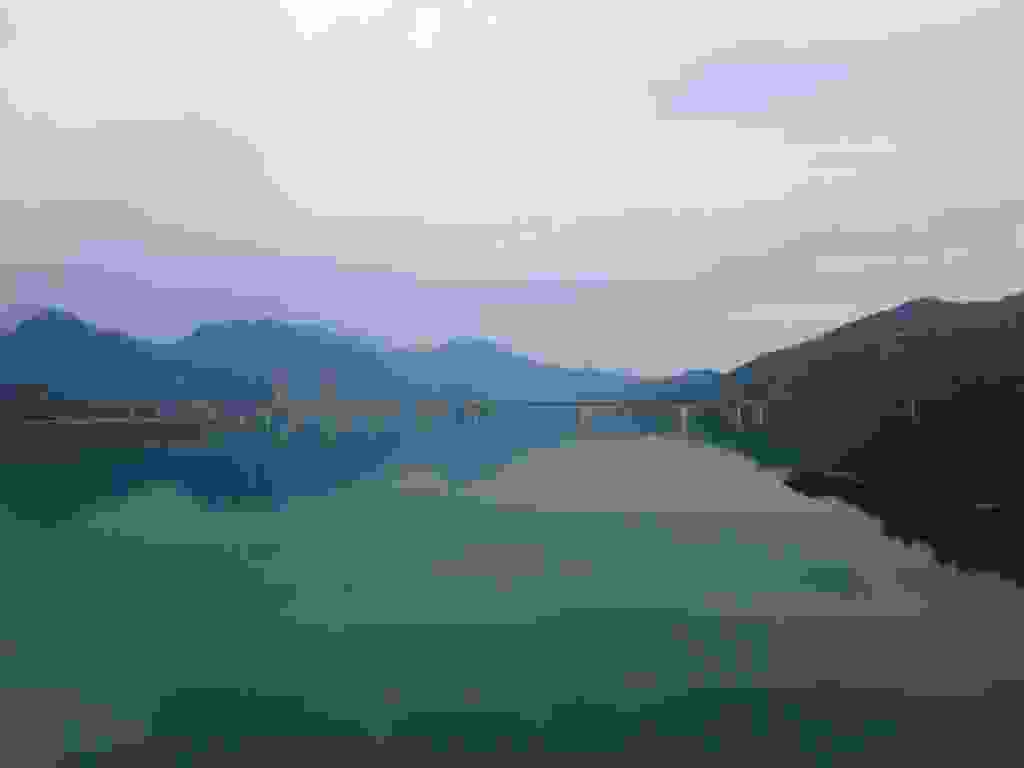
\includegraphics[width=\mywidth]{../wp-content/uploads/2015/09/wpid-p91970172-1024x768.jpg} } 
 \newline
 Je visite le système d'irrigation de Dujiangyian construit il y a plus de 2000 ans \newline
 \newline
\centerline{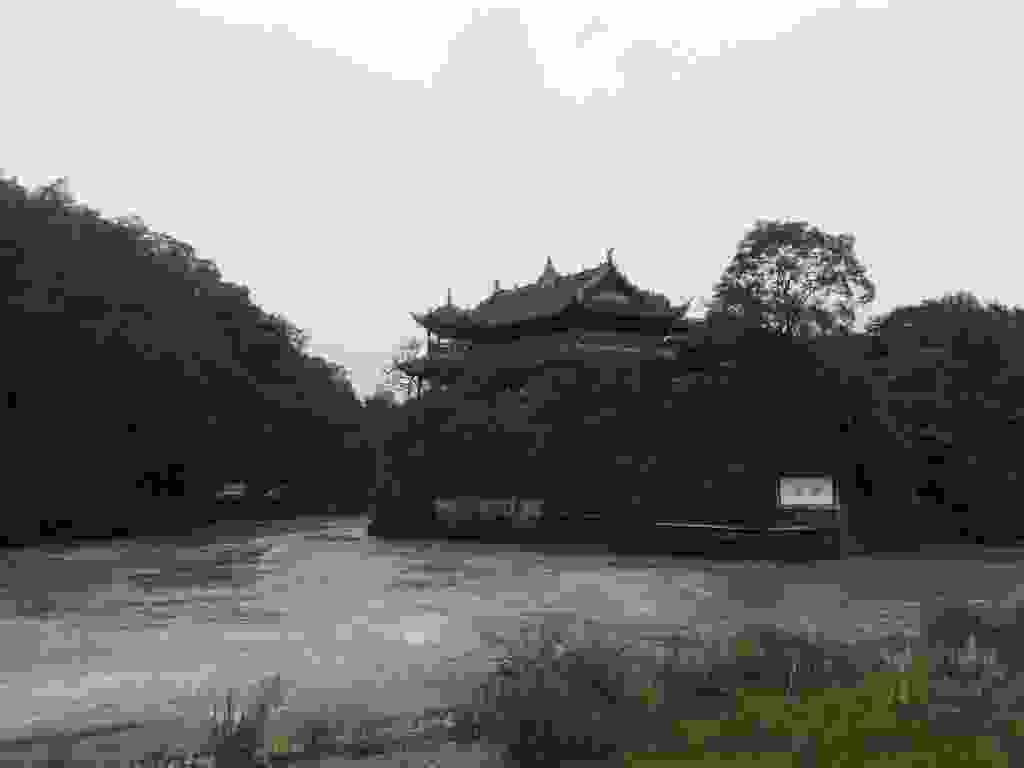
\includegraphics[width=\mywidth]{../wp-content/uploads/2015/09/wpid-p9207025-1024x768.jpg} } 
 \newline
 \newline
\centerline{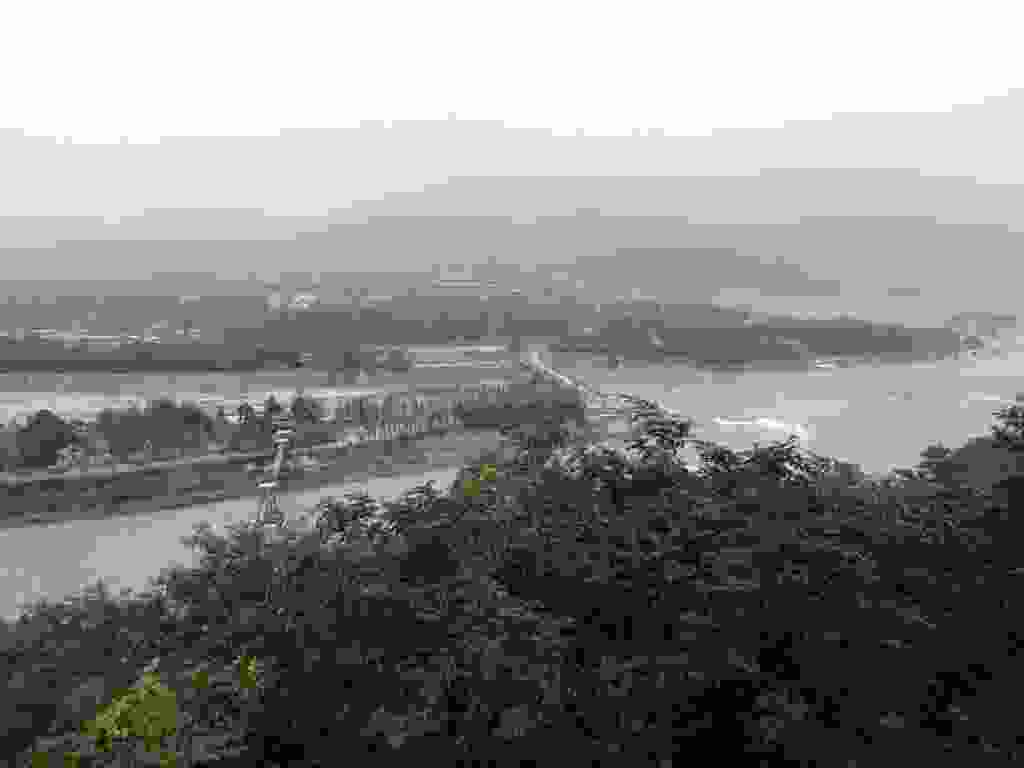
\includegraphics[width=\mywidth]{../wp-content/uploads/2015/09/wpid-p9207031-1024x768.jpg} } 
 \newline
 \newline
\centerline{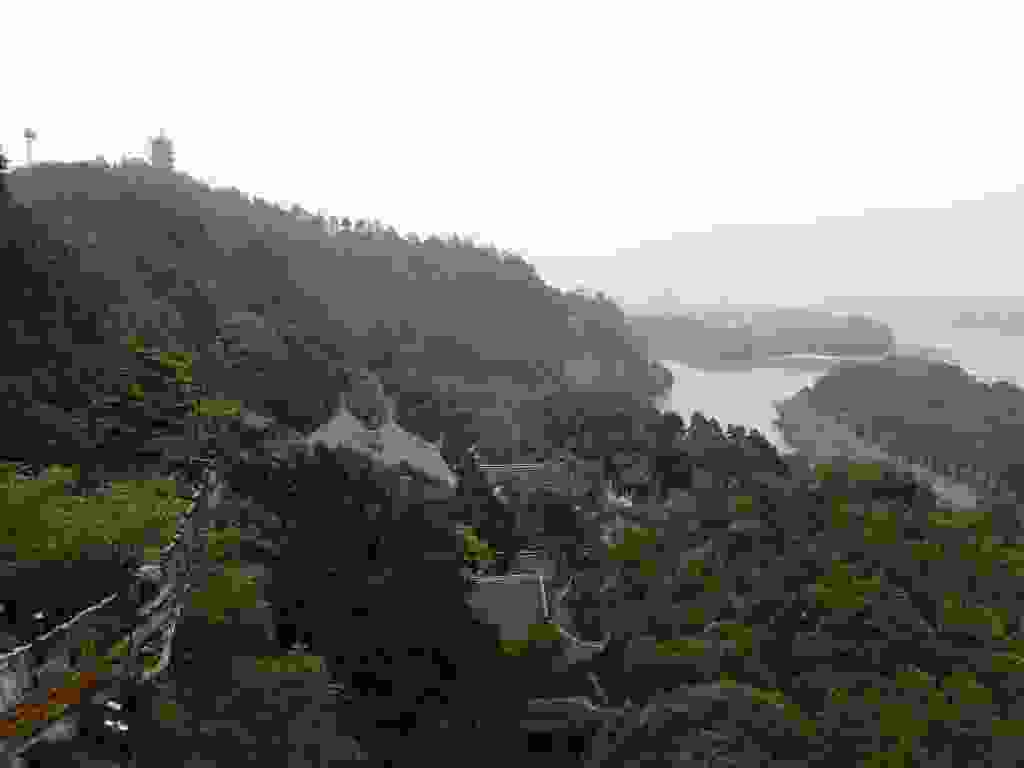
\includegraphics[width=\mywidth]{../wp-content/uploads/2015/09/wpid-p9207032-1024x768.jpg} } 
 \newline
 A quelques km le mont Qingcheng et ses temples taoïstes, il faisait vraiment moche je me suis contenté du premier temple en bas \newline
 \newline
\centerline{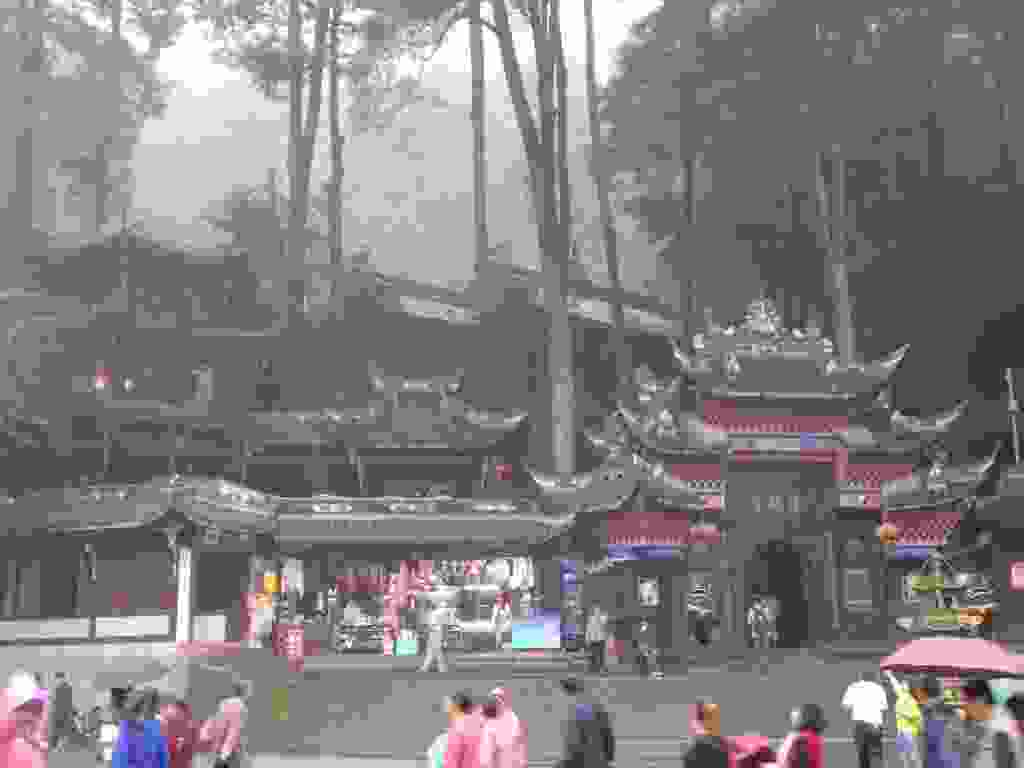
\includegraphics[width=\mywidth]{../wp-content/uploads/2015/09/wpid-p9207048-1024x768.jpg} } 
 \newline
 \newline
\centerline{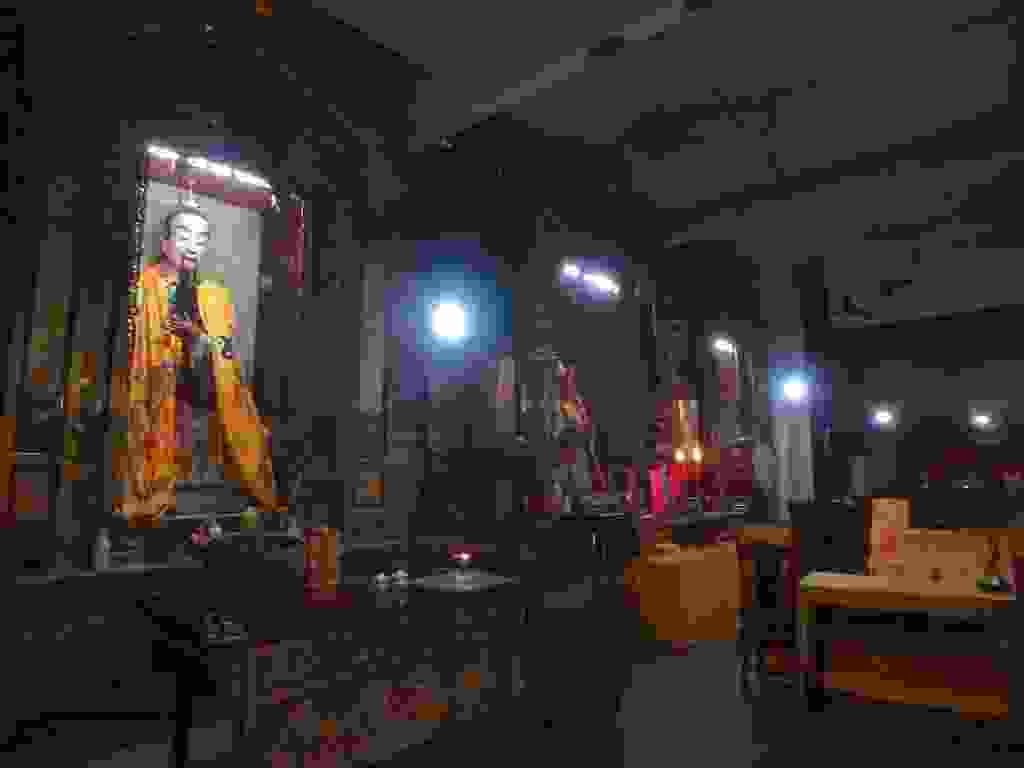
\includegraphics[width=\mywidth]{../wp-content/uploads/2015/09/wpid-p9207047-1024x768.jpg} } 
 \newline
 Les pandas, symboles du Sichuan, à l'entrée de Chengdu \newline
 \newline
\centerline{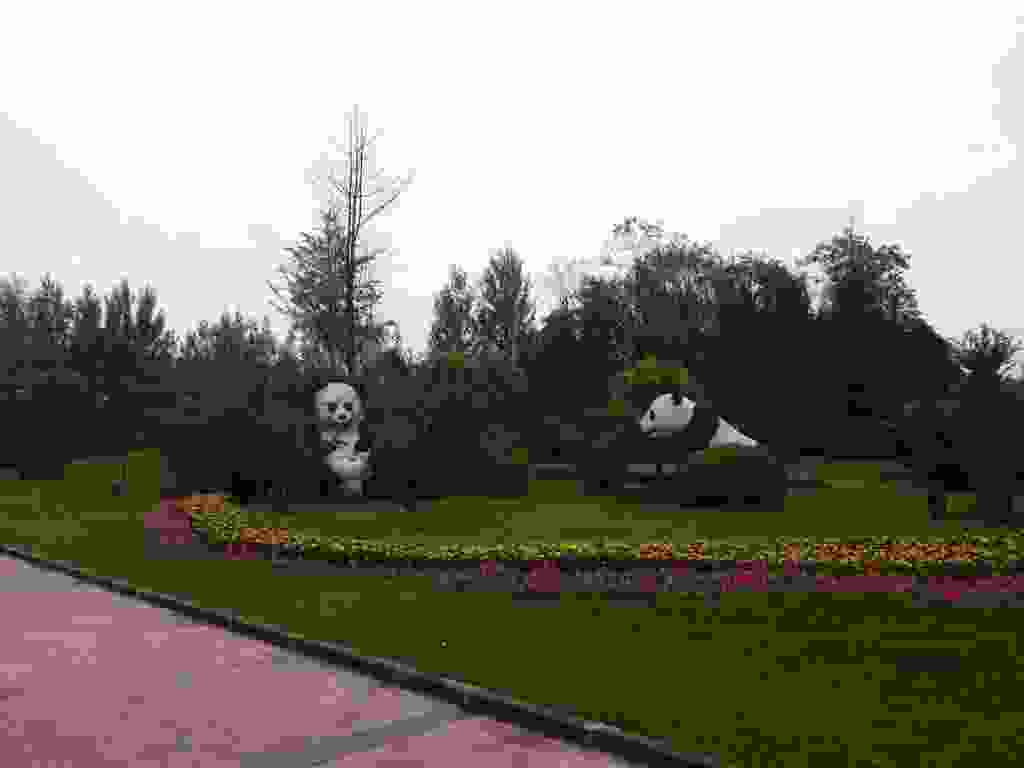
\includegraphics[width=\mywidth]{../wp-content/uploads/2015/09/wpid-p92170512-1024x768.jpg} } 
 \newline
 Cuisine bien pimentée dans le Sichuan, plat à base de poulet et cacahuètes que j'ai retrouvé plusieurs fois \newline
 \newline
\centerline{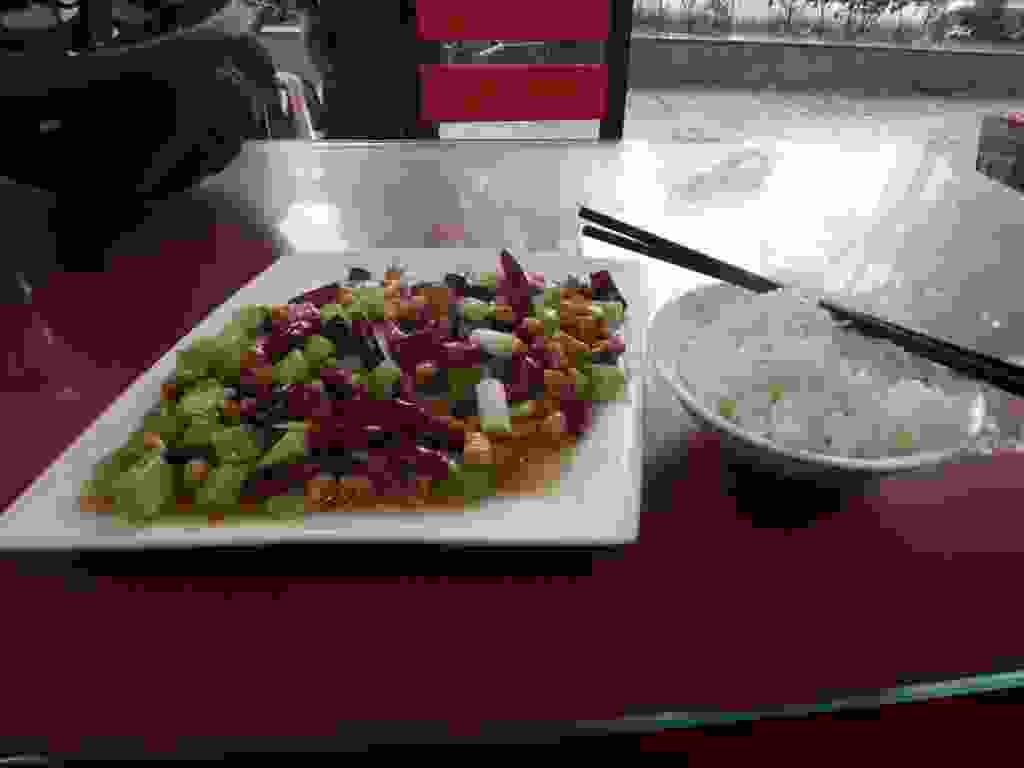
\includegraphics[width=\mywidth]{../wp-content/uploads/2015/09/wpid-p9207045-1024x768.jpg} } 
 \newline

\newpage
 
